% !TeX spellcheck = en
\documentclass[preprint,svgnames]{iacrtrans}

\usepackage[utf8]{inputenc}
\usepackage{amssymb, amsmath, amsfonts, amscd}
\usepackage[T1]{fontenc}
\usepackage{graphicx}
\usepackage{url}
\usepackage{xspace}
\usepackage{subcaption}
\usepackage{algorithm}
\usepackage{tikz}
\usepackage{cellspace}
\usepackage{multirow}
%\usepackage{parskip}
\usetikzlibrary{patterns}

%\usepackage[noend]{algpseudocode}

%\usepackage[pdftex,bookmarks,bookmarksopen,bookmarksdepth=3]{hyperref}
%\hypersetup{colorlinks=true,citecolor=red,linkcolor=red,urlcolor=black}

\DeclareMathSymbol{:}{\mathord}{operators}{"3A}
\DeclareMathOperator{\LCG}{LCG}
\DeclareMathOperator{\MCG}{MCG}

\usepackage[noend]{algpseudocode}
%\usepackage{algorithmic}

% knuth-style algos
% \newcommand{\slug}{\hbox{\kern1.5pt\vrule width2.5pt height6pt depth1.5pt\kern1.5pt}}
% \def\xskip{\hskip 7pt plus 3pt minus 4pt}
% \newdimen\algindent
% \newif\ifitempar \itempartrue % normally true unless briefly set false
% \def\algindentset#1{\setbox0\hbox{{\bf #1.\kern.25em}}\algindent=\wd0\relax}
% \def\algbegin #1 #2{\algindentset{#21}\alg #1 #2} % when steps all have 1 digit
% \def\aalgbegin #1 #2{\algindentset{#211}\alg #1 #2} % when 10 or more steps
% \def\aaalgbegin #1 #2{\algindentset{#2111}\alg #1 #2} % when 10 or more steps
% \def\alg#1(#2). {\medbreak % Usage: \algbegin Algorithm A (algname). This...
%   \noindent{\bf#1}({\it#2\/}).\xskip\ignorespaces}
% \def\algstep#1.{\ifitempar\smallskip\noindent\else\itempartrue
%   \hskip-\parindent\fi
%   \hbox to\algindent{\bf\hfil #1.\kern.25em}%
%   \hangindent=\algindent\hangafter=1\ignorespaces}
% end of borrowed macros

\newcommand{\todo}[1]{\textcolor{red}{TODO:[#1]}}

\title{Predicting the PCG PSeudo-Random Number Generator In Practice} 

\author{Charles Bouillaguet\inst{1} \and Julia Sauvage\inst{2} \and Florette Martinez\inst{3}}


\institute{% 
University of Lille, France \\ 
\email{charles.bouillaguet@univ-lille.fr}
\and 
Sorbonne University \\
\email{julia.sauvage@etu.upmc.fr}
\and 
LIP6, CNRS, SU ? \\
\email{florette.martinez@lip6.fr}

}

\begin{document}
\maketitle

\keywords{keywords}

\begin{abstract}
  blablabla
\end{abstract}

\section{Introduction} %ce qu'on avait écrit pour le projet, peut-être pas incroyable...

\todo{Ca, c'est du blabla...}

Pseudo-random generators (PRG) are well-studied primitives in symmetric
cryptography. A PRG is an efficient deterministic algorithm that stretch a small
random seed into a longer pseudo-random stream. To achieve cryptographic-grade
pseudo-randomness, a PRG must ensure that the pseudo-random stream is
computationally indistinguishable from a ``truly'' random sequence of bits by
efficient adversaries. Alternatively, it is possible to define pseudo-randomness
by asking that no efficient algorithm is capable of predicting the next
pseudo-random bit with non-negligible accuracy. The two definitions are in fact
equivalent.

\todo{mentioner stream ciphers}

Not all pseudo-random generators are of cryptographic strength. In some
applications, it is not necessarily necessary: to be used in Monte-Carlo
simulations or generate random choices in games, a relaxed, non-cryptographic
notion of pseudo-randomness may be sufficient. This allows for faster
algorithms. For instance, the \texttt{Math.Random} function in Google's V8
open-source JavaScript engine uses the \textsf{XorShift128} generator, which is
a Linear Feedback Shift Register tailored for high software speed. On 64-bit
processors, it produces 64 pseudo-random bits with 3 shifts and 4 XORs
instructions. The \textsf{python} standard library's \texttt{random} module uses
the Mersenne Twister. The \textsf{C} library that comes along \texttt{gcc} (the
\texttt{glibc}) uses a (poor) truncated linear congruential generator by default
to implement the \texttt{rand} function.

In the realm of non-cryptographic random generators, a PRG is deemed ``good
enough'' it is passes \emph{some} efficient statistical tests --- whereas the
cryptographic notion of pseudo-randomness asks that it passes \emph{any}
efficient test. There are \textit{de facto} statistical test suites (\todo{les
  mentionner}). The goal of designers then consists in designing the fastest
possible generator that passes the day's favourite test suite.

\todo{Mentionner Ferrenberg 92}

The scientific computing community also realized that the need for fast
\emph{parallel} random number generation could be satisfied by the use of block
ciphers in counter mode~\cite{Salmon11}. The need for speed then leads to the
use of weakened cryptographic primitives.

In most cases, it is easy to see that a non-cryptographic PRG does not meet the
cryptographic notion of pseudo-randomness, and there are few exceptions. In this
paper, we study the \textsf{PCG} family of non-cryptographic pseudo-random
generators~\cite{melissapaper,melissaweb}.

\textsf{PCG} stands for ``Permuted Congruential Generator'': it essentially
consists in applying a non-linear filtering function on top of a (fairly weak)
linear congruential generator (in a way reminiscent to the venerable filtered
LFSRs). The resulting combination is fast and passes current test suites. Its
designer claimed that distinguishing the pseudo-random stream produced would be
``challenging''. The \textsf{PCG} family contains many members, but we focus on
its strongest member, named either \textsf{PCG64} or \textsf{PCG-XSL-RR}. It has
a 128-bit internal state and produces 64 bits when clocked. It is the default
pseudo-random number generator in the popular \textsf{NumPy} scientific
computing package for \textsf{Python}.

The internal state of the \textsf{PCG64} generator is made of a 128-bit
``state'' and a 128-bit ``increment'', whose intended use is to provide several
pseudo-random streams with the same seed (just as the initialisation vectors do
in stream ciphers). A default increment is provided in case the end-user just
want one pseudo-random stream with a single 128-bit seed.

\paragraph{Contribution.} We describe an algorithm that reconstructs the full
internal state of the strongest member of the \textsf{PCG} family. This allows
to predict the pseudo-random stream deterministically and clock the generator
backwards. The original seeds can also easily be reconstructed. The algorithm is
practical and we have executed it in practice. It follows that predicting the
output of the \textsf{PCG} should not be considered challenging anymore.

Our algorithm reconstruct the internal state using the ``guess-and-determine''
technique: some bits of the internal state are guessed ; assuming the guesses
are correct, some other information is computed ; a consistency check discards
bad guesses early on ; then candidate internal states are computed and fully
tested. The problem actually come in two distinct flavors.

When the increment is known (for instance when it is the default value), a
simplified prediction algorithm recovers the internal state from 192 bits of
pseudo-random stream. The process runs in 20 CPU minutes (on a single core of a
server processor). It guesses 36 bits of the internal state, then solves an
instance of the \textsc{Closest Vector Problem} (CVP) in a 3-dimensional
euclidean lattice. This requires about 50 arithmetic operations in total and
reveals the entire internal state if the guesses are correct.

When the increment is unknown, things are a bit more complicated. This is the
default situation in \textsf{NumPy}, where both the state and the increment are
initialised using an external source of entropy. In this case, our prediction
algorithm requires 3072 bits of pseudo-random stream ; it guesses between 51 and
55 bits, then for each guess it solves and instance of CVP in dimension 4 (using
about 75 arithmetic operations). This recovers 64 more bits of information about
the difference between two successive states, and this is enough to filter the
bad guesses. This information can then be used in a subsequent and comparably
inexpensive phase to recover the entire internal state. On average, the whole
process requires a bit less than 20 000 CPU hours to complete.

We implemented the algorithms in \textsf{C}, then asked the designer of the PCG
family to send us ``challenge'' pseudo-random streams ; we ran our code and
emailed back the seeds used to generate the challenge streams the next day.

\paragraph{Related Work.} \todo{Mentionner Knuth et les LCG + Frieze + Boyar + Stern...}

\todo{mentionner Vigna ?}

% The combination between being highly commended (it achieved 5th place out of 29
% in a recent performance test survey\cite{survey}) and a well presented
% website\cite{melissaweb} giving an feeling of professionalism can lead to the
% impression that PCG is a sufficiently secure family of generators.

% Some attacks against PCG have been carried out by Sebastiano
% Vigna\cite{vignaweb}, but this didn't yield any significant results, given that
% he only tried to break an incomplete version in a fairly straightforward way. He
% worked on a very specific version of PCG. He considers the result without
% modulo, which is a big simplification. Moreover, he didn't study the 128 bits
% long generator, but only the 64 bits long\cite{vignacode}.


\section{The PCG Pseudo-Random Number Generator Family}

This section describes the \textsf{PCG64} non-cryptographic pseudo-random number
generator (more precisely \textsf{PCG-XSL-RR} in the designer's terminology). It
has an internal state of 128-bit, which operate as a linear congruential
generator modulo~$2^{128}$. More precisely:
\[
  S_{i+1} = a S_i + c \bmod 2^{128},
\]
Where $a = 47026247687942121848144207491837523525$ is a fixed 126-bit
constant. The first initial state $S_0$ is the seed of the generator. The
increment $c$ may be specified by the user of the PRNG to produce different
output streams with the same seed (just as the IV acts in a stream cipher). If
no value of $c$ is specified, then a default increment is provided:
$c = 117397592171526113268558934119004209487$. Note that $c$ must be odd.

Each time the PRNG is clocked, 64 output bits are extracted from the internal
state using a non-linear function that makes use of data-dependent rotations, in
a way reminiscent of the \textsf{RC5} block cipher~\cite{Rivest94}. The six most
significant bits of the internal state encode a number $0 \leq r < 64$. The two
64-bit halves of the internal state are XORed together, and this 64-bit result
is rotated right by $r$ positions. The successive 64-bit outputs of the
generator are $X_0, X_1, \dots$ where:
\begin{equation}\label{eq:output}
  X_i =(S_i[0:64] \oplus S_i[64:128]) \ggg S_i[122:128].
\end{equation}

Figure~\ref{pcg128out} summaries the process. The overall design strategy is
similar to that of a filtered LFSR: the successive states of a weak internal
generator with a strong algebraic structure are ``filtered'' by a non-linear
function.

Updating the internal state requires a $128 \times 128 \rightarrow 128$
multiplication operation. In fact, this can be done with two
$64 \times 64 \rightarrow 64$ multiplications, one
$64 \times 64 \rightarrow 128$ multiplication and two 64-bit additions. High-end
desktop CPUs all implement these operations in hardware, so the generator is
relatively fast on these platforms.


\begin{figure}
  \begin{center}
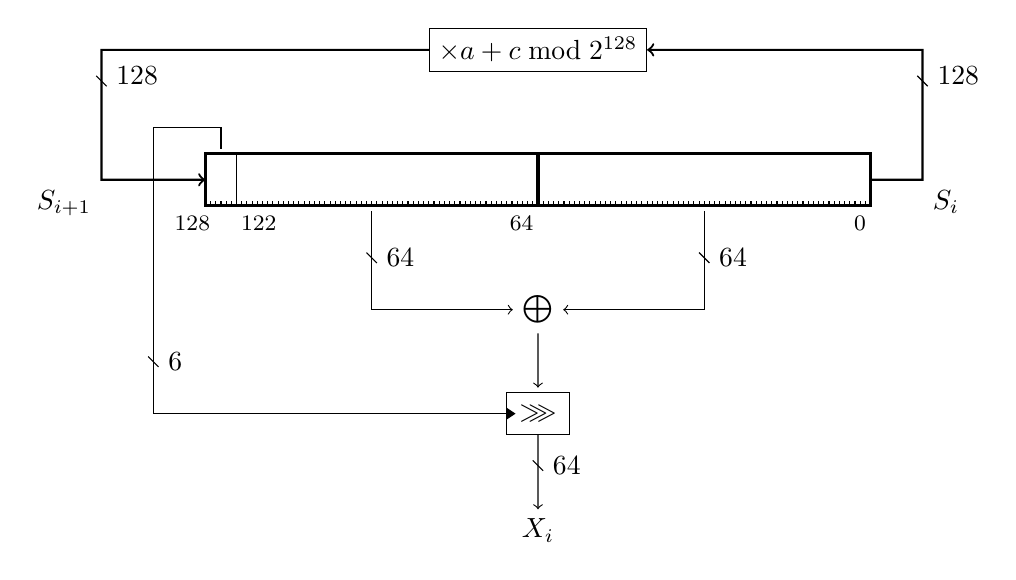
\begin{tikzpicture}[scale=0.66]
%  \draw[red, use as bounding box] (-1.25, -6.75) rectangle (12.8, 2.25);
  
  % S_i

    % bordures
    \draw[very thick]  (0, 0) rectangle (12.8, 1);
    \draw  (0.6, 0) rectangle +(0, 1);
    \draw[very thick]  (6.4, 0) rectangle +(0, 1);
    \foreach \i in {0, 1, ..., 128} \draw (\i/10, 0) -- +(0, 0.1);
    
    % déco autour
    \node[draw] at (6.4, 3) (update) {$\times a + c \bmod 2^{128}$};
    \draw[thick,->] (12.8, 0.5) -- (13.8, 0.5) node[below right] {$S_i$} -- (13.8, 3) -- (update);
    \draw (13.7, 2.5) -- +(0.2, -0.2);
    \path (13.9, 2.5) node[anchor=west] {128};

    \draw[thick,->] (update) -- (-2, 3) -- (-2, 0.5) node[below left] {$S_{i+1}$} -- (0, 0.5);
    \draw (-2.1, 2.5) -- +(0.2, -0.2);
    \path (-1.9, 2.5) node[anchor=west] {128};

    
    \node[font=\footnotesize,anchor=east] at (12.9, -0.33) {0};
    \node[font=\footnotesize,anchor=east] at (6.5, -0.33) {64};
    \node[font=\footnotesize,anchor=west] at (0.5, -0.33) {122};
    \node[font=\footnotesize] at (-0.25, -0.33) {128};
    
    \draw (6.4, -2) node (x) {$\bigoplus$};
    
    \draw[->] (3.2, -0.1) |- (x);
    \draw (3.1, -0.9) -- +(0.2, -0.2);
    \path (3.3, -1) node[anchor=west] {64};
    
    \draw[->] (9.6, -0.1) |- (x);
    \draw (9.5, -0.9) -- +(0.2, -0.2);
    \path (9.7, -1) node[anchor=west] {64};

    \node[minimum width=1.8cm] at (6.4, -4) (r) {$\ggg$};
    \draw (5.8, -3.6) rectangle +(1.2, -0.8);
    \draw[fill=black] (5.8, -4.1) -- (5.95, -4) -- (5.8, -3.9) -- cycle;
    
    \draw (0.3, 1.1) -- (0.3, 1.5) -- (-1, 1.5) -- (-1, -4) -- (5.8, -4);
    \draw (-1.1, -2.9) -- +(0.2, -0.2);
    \path (-0.9, -3) node[anchor=west] {6};

    \draw[->] (x) -- +(0, -1.5);
    \node at (6.4, -6.25) (xi) {$X_i$};
    \draw[->] (6.4, -4.4) -- (xi);

    \draw (6.3, -4.9) -- +(0.2, -0.2);
    \path (6.5, -5) node[anchor=west] {64};
  \end{tikzpicture}
\end{center}
\caption{\textsf{PCG64}: Internal state update and output process.}
\label{pcg128out}
\end{figure}


\section{Reconstructing Truncated Geometric Sequences}
\label{sec:geometric}

\subsection{Reconstructing Linear Congruential Generators}

Given an integer \(k\), a fixed multiplier \(a\) and an increment \(c\), define the
sequence \[u_0 = x, u_{i+1} = a u_i + c \bmod 2^k\] The sequence \(u\) form the
successive internal states of a linear congruential generator (LCG). 

Let $\LCG_{n,k}(x, c)$ denote the vector $(u_0, \dots, u_{n-1}) \in \mathbb{Z}_{2^k}$ (we will omit $n$ and $k$ when they are obvious from the context).  It is easy to check that:
\begin{align}
\label{eq:lcg-additive}
\LCG_{n,k}(x + y, c + d) &= \LCG_{n,k}(x, c) + \LCG_{n,k}(y, d),  \\
\label{eq:lcg-scalar}
\LCG_{n,k}(\lambda x, \lambda c) &= \lambda \LCG_{n,k}(x, c).   
\end{align}
Hence those sets of vector have a lot of structure we can use.

The LCG have been largely studied. This is why we know techniques to recover internal states knowing only upper or lower bits of the output, see \cite{Boyar1989}. A particular LCG is the Lehmer's generator \cite{Lehmer}, where the multiplier \(a\) is known and the increment is zero.

In our algorithm to predict the PCG, we need to reconstruct several truncated Lehmer's generator. For that, we will present a classical lattice-based reconstruction for a truncated Lehmer's generator, as presented in \cite{Frieze}. \todo{C'est pas exactement celle là, on dit quoi du coup ?}

\subsection{The lattice associated to a Lehmer's generator}

We fix a multiplier \(a\), integers \(k\), \(n\) and we consider \(L(n,k)\) the set of \(\LCG_{n,k}(x, 0)\), for \(x\) in \(\mathbb{Z}_{2^k}\). Then

\begin{itemize}
	\item By \ref{eq:lcg-additive}, the vector \(\LCG(x_1,0) + \LCG(x_2,0) = \LCG(x_1+x_2,0)\), hence it is still in \(L(n,k)\).
	\item By \ref{eq:lcg-scalar}, the vector \((-1)\times \LCG(x,0) = \LCG(-x,0)\) hence it is still in \(L(n,k)\).
\end{itemize}

Hence \(L(n,k)\) is a lattice. We easily notice that \(L(n,k)\) is spawned by the lines of the following \(n\times n\) matrix :

\[\begin{pmatrix}
1&a&a^2&\dots&a^{n-1}\\
0&2^k&0&\dots&0\\
0&0&2^k&\dots&0\\
\dots&\dots&\dots&\dots&\dots\\
0&0&0&\dots&2^k\\
\end{pmatrix}\]

Once again, we will omit $n$ and $k$ when they are obvious from the context.

We want to find an element \(U\) in the lattice only knowing the most significant bits of each of its coordinates. 

We decompose \(U = T + (T-U)\) where \(T\) contains only the upper bits and \(T-U\) the lowers one. There is no reason for \(T\) to be in the lattice, but as \(T-U\) is small, we know \(T\) is \emph{close} to \(U\).

\subsection{A first way to find U : using an exact CVP solver}

Solving exactly the CVP is a hard computational problem. The algorithms used are costly, but we can afford to use them up to dimension 50.

We know that \(U\) is in the lattice, \(T\) is usually not and \(|T-U|\) is small. Then we can hope for \(U\) to be the closet vector of \(T\) which is in the lattice : the vector \(U\) may be the solution of \(CVP(L,T)\).

What can we say about \(|CVP(L,T)-U|\) ?

\begin{align*}
|CVP(L,T)-U| &= |CVP(L,T)-T+T-U|\\
& \leqslant |CVP(L,T)-T|+|T-U|\\
\end{align*}

But, as the vector \(U\) is in the lattice and by definition of the CVP, \(|CVP(L,T)-T| \leqslant |T-U| \), hence 
\[|CVP(L,T)-U|\leqslant 2|T-U|\]

If we can prove that the right side of the inequality is smaller than first minimum of the lattice \(\lambda_1(L)\), then we have proved that \(CVP(L,T)\) is indeed the vector we were searching for.

In this article, we will only use the Babai's rounding when \(k = 128-\ell\) and when we know the \(6\) upper bit of our Lehmer's generator. Hence \(\lVert T-U \rVert \leqslant \sqrt{n}2^{122-\ell} \). So, if we fix \(\ell\) we can search for the minimum \(n\) such that \[2\sqrt{n}2^{122-\ell} \leqslant \lambda_1(L(128-\ell,n))\].

\begin{table}
  \centering
    \begin{tabular}{|c|c|}
	\hline
	\(\ell\)  & minimum \(n\) \\
	\hline
	11 & 39 \\
	12 & 38 \\
	13 & 38 \\
	\hline
\end{tabular}
  \caption{\todo{WRITE-ME}}
  \label{tab:exact_cvp}
\end{table}

\subsection{A second way to find U : the Babai's rounding}

As using an exact CVP solver is costly, we'll try a cheaper but less precise way to find the closest vector.

We compute \(G(n,k)\) the LLL-reduction of the generating matrix of \(L(n,k)\). We denote by  \(\rVert G \lVert\) the induced matrix norm :
\[\rVert G \lVert =  \max_{x \in \mathbb{R}}\frac{\lVert Gx \rVert_2}{\lVert x \rVert_2}\]
In the case of the \(\lVert\rVert_2\) norm, \(\rVert G \lVert = \sigma(G)\), where \(\sigma(G)\) is the largest singular value of \(G\). 

\medskip

As \(T\) is not an element of the lattice, \(TG^{-1}\) is not an integer vector.

We fix \(r = rounding(TG^{-1}) \), then \(rG\) is an element of the lattice. What can we say about the distance between \(rG\) and \(U\) ?

\begin{align*}
\lVert U - rG \rVert &= \lVert U - (r-TG^{-1} + TG^{-1})G \rVert\\
&= \lVert U - T + (r-TG^{-1})G \rVert\\
&\leqslant \lVert U - T \rVert + \lVert(r-TG^{-1})\rVert \times \lVert G\rVert\\	
\end{align*}

By definition, \(r\) is the closest integer vector to \(TG^{-1}\). But as \(U\) is an element of the lattice, \(UG^{-1}\) is an integer vector. Thus \(r-TG^{-1}\) is shorter than \(UG^{-1}-TG^{-1}\).

Hence :
\begin{align*}
\lVert U - rG \rVert &\leqslant \lVert U - T \rVert + \lVert(r-TG^{-1})\rVert \times \lVert G\rVert\\	
&\leqslant \lVert U - T \rVert + \lVert(UG^{-1}-TG^{-1})\rVert \times \lVert G\rVert\\	
&\leqslant \lVert U - T \rVert + \lVert(U-Y)\rVert \times \lVert G^{-1} \rVert  \times \lVert G\rVert\\
& 	\leqslant \lVert U - T \rVert \times (1 +\lVert G^{-1} \rVert  \times \lVert G\rVert )\\
\end{align*}

If we can prove that the right side of the inequality is smaller than the minimum of the lattice \(\lambda_1(L)\), then we have proved that \(rG\) is indeed the vector we were searching for.

In this article, we will only use the Babai's rounding when \(k = 64\) and when we know the \(6+\ell\) upper bit of our Lehmer's generator. Hence \(\lVert T-U \rVert \leqslant \sqrt{n}2^{58-\ell} \). So, if we fix \(n\) we can search for the minimum \(\ell\) such that \[(1+\lVert G(n,64) \rVert \times \lVert G(n,64)^{-1} \rVert)\sqrt{n}2^{58-\ell} \leqslant \lambda_1(L(n,64))\]

\bigskip

\begin{table}
  \centering
  \begin{tabular}{|c|c|c|c|}
	\hline
	n & \(\lVert G(n,64) \rVert \times \lVert G(n,64)^{-1} \rVert\) & \( \lambda_1(L(n,64)) \) & minimum \(\ell\) \\
	\hline
	3 & 2.869065991049632 & \(4.08909120094543e^{12}\) & 19 \\
	4 & 2.060717188416003 & \(2.43569932844650e^{14}\) & 13 \\
	5 & 3.7692142154392747 & \(1.71669732658884e^{15}\) & 11 \\
	6 & 2.6925925483728537 & \(1.02550589786192e^{16}\) & 8 \\
	\hline
  \end{tabular}
  \caption{\todo{WRITE-ME}}
  \label{tab:babai}
\end{table}

\section{Warm-up: A Prediction Algorithm for \textsf{PCG64} With Known Increment}
\label{sec:Cknown}

We first consider the easier case where the ``increment'' (the $c$ term in the
definition of the underlying linear congruential generator) is known --- recall
that a default value is specified in case the user of the pseudo-random
generator does not want to provide one.

In this case, reconstructing the 128-bit internal state $S_i$ of the generator
is sufficient to produce the pseudo-random flow with 100\% accuracy (the
generator can also be clocked backwards if necessary, so that the seed can be
easily reconstructed). We therefore focus on reconstructing $S_0$ (the seed)
from $X_0, X_1, X_2, \dots$. A very simple strategy could be the following:
\begin{enumerate}
\item Guess the 64 upper bits of $S_0$.
\item Compute the missing 64 lower bits using~\eqref{eq:output}, with:
\[
   S_0[0:64] = S_0[64:128] \oplus (X_0  \lll S[122:128]).
\]
\item If $X_1$ is computed correctly, then output $S_0$.
\end{enumerate}

This ``baseline'' procedure requires $2^{64}$ iterations of a loop that does a
dozen arithmetic operations; it always output the correct value of $S_0$, and
may output a few other ones (they can be easily discarded by checking $X_2$). An
improved ``guess-and-determine'' prediction algorithm is possible, which
essentially amounts to expose a truncated version of the underlying linear
congruential generator, and attack it using the well-known tools. This is
possible by combining the following ingredients:
\begin{itemize}
\item The underlying linear congruential generator uses a power-of-two modulus,
  therefore the $\ell$ low-order bits of $S_{i+1}$ are entirely determined by
  the $\ell$ low-order bits of $S_i$. More precisely, we have:
  \begin{equation}\label{eq:lcg}
    S_{i+1} = aS_i + c \bmod 2^\ell, \qquad \text{for all } 0 \leq \ell \leq 128
  \end{equation}
  Therefore, guessing low-order bits of $S_0$ yields a ``long-term advantage''
  that holds for all subsequent states.

\item Guessing a 6-bit rotation gives access to the XOR of the two halves of the
  internal state. If a part of the state is known, then this transfers existing
  knowledge to the other half.
\end{itemize}

In figure~\ref{fig:Cknown}, we see that guessing $S_0[0:\ell]$ and a few 6-bit
rotations give access to $S_i[58:64+\ell]$ for the corresponding
states. Therefore, looking at $S_i[\ell:64+\ell]$, we are facing a truncated
linear congruential generator on $64$ bits, where we have access to the most
$6+\ell$ bits of each state (denoted by $T$), for a few consecutive states. This
is sufficient to reconstruct entirely the successive states of this truncated
linear congruential generator. This reveals $S_0[\ell:64+\ell]$, and
using~\eqref{eq:output} the entire $S_0$ can be reconstructed. The precise
details follow.

\begin{figure}
\begin{center}
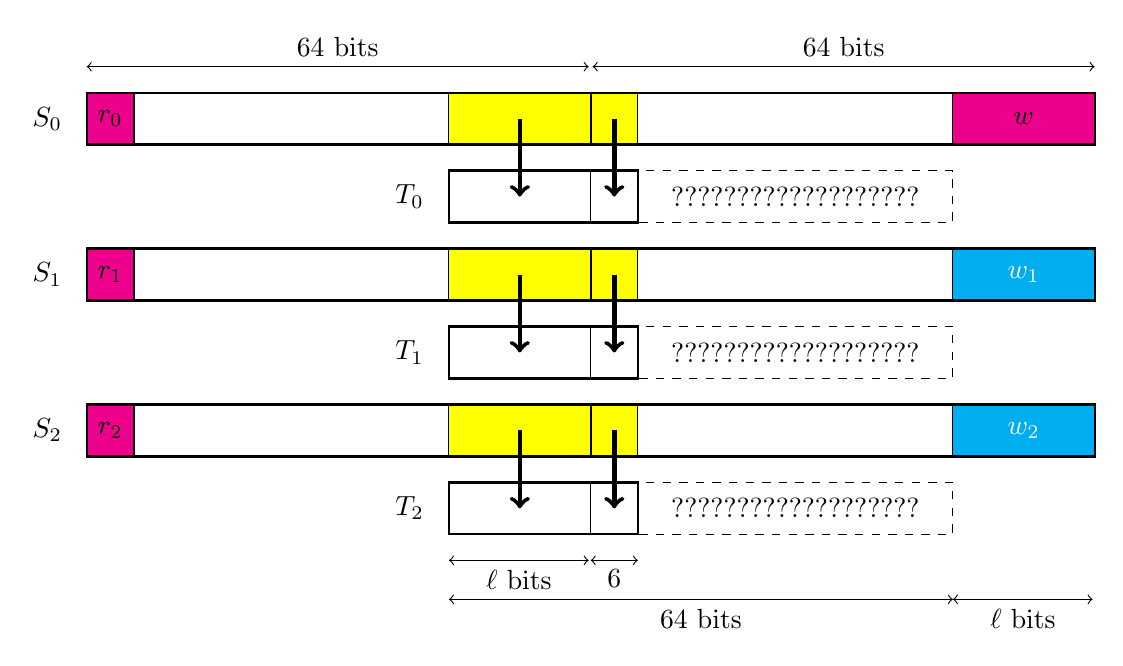
\begin{tikzpicture}[yscale=0.66]
  \path[red, use as bounding box] (-0.75, -9.5) rectangle (12.8, 2.25);
  
  % S_0
  \begin{scope}
    % remplissage
    \fill[fill=Yellow] (4.6, 0) rectangle +(2.4, 1);
    \fill[fill=magenta] (0, 0) rectangle node {$r_0$} +(0.6, 1);
    \fill[fill=magenta] (11, 0) rectangle node {$w$} +(1.8, 1);
    
    % bordures
    \draw[thick]  (0, 0) rectangle (12.8, 1);
    \draw  (0.6, 0) rectangle +(0, 1);
    \draw[thick]  (6.4, 0) rectangle +(0, 1);
    \draw  (7.0, 0) rectangle +(0, 1);
    \draw  (4.6, 0) rectangle +(0, 1);
    \draw  (11, 0) rectangle +(0, 1);
    
    % déco autour
    \node at (-0.5, 0.5) {$S_0$};
    \draw[<->] (0, 1.5) -- node[above] {64 bits} +(6.375, 0);
    \draw[<->] (6.425, 1.5) -- node[above] {64 bits} +(6.375, 0);
  \end{scope}

  % T_0
  \begin{scope}[xshift=4.6cm, yshift=-1.5cm]    
    \draw[dashed]  (0, 0) rectangle +(6.4, 1);
    \draw[thick]  (0, 0) rectangle +(2.4, 1);
    \draw[]  (1.8, 0) rectangle +(0, 1);
    \path (2.4, 0) rectangle node {$???????????????????$} (6.4, 1);

    % déco
    \node at (-0.5, 0.5) {$T_0$};
  \end{scope}

  % flèches S_i --> T_i
  \draw[ultra thick,->] (5.5, 0.5) -- +(0, -1.5);
  \draw[ultra thick,->] (6.7, 0.5) -- +(0, -1.5);

  
  %%%%%%%%%

  
  % S_1
  \begin{scope}[yshift=-3cm]
    % remplissage
    \fill[fill=Yellow] (4.6, 0) rectangle +(2.4, 1);
    \fill[fill=magenta] (0, 0) rectangle node {$r_1$} +(0.6, 1);
    \fill[fill=cyan] (11, 0) rectangle node[text=white] {$w_1$} +(1.8, 1);
    
    % bordures
    \draw[thick]  (0, 0) rectangle (12.8, 1);
    \draw  (0.6, 0) rectangle +(0, 1);
    \draw[thick]  (6.4, 0) rectangle +(0, 1);
    \draw  (7.0, 0) rectangle +(0, 1);
    \draw  (4.6, 0) rectangle +(0, 1);
    \draw  (11, 0) rectangle +(0, 1);
    
    % déco autour
    \node at (-0.5, 0.5) {$S_1$};

    % flèches S_i --> T_i
    \draw[ultra thick,->] (5.5, 0.5) -- +(0, -1.5);
    \draw[ultra thick,->] (6.7, 0.5) -- +(0, -1.5);
  \end{scope}

  % T_1
  \begin{scope}[xshift=4.6cm, yshift=-4.5cm]    
    \draw[dashed]  (0, 0) rectangle +(6.4, 1);
    \draw[thick]  (0, 0) rectangle +(2.4, 1);
    \draw[]  (1.8, 0) rectangle +(0, 1);
    \path (2.4, 0) rectangle node {$???????????????????$} (6.4, 1);

    % déco
    \node at (-0.5, 0.5) {$T_1$};
  \end{scope}

  %%%%%%%%%%%%%

  
  % S_2
  \begin{scope}[yshift=-6cm]
    % remplissage
    \fill[fill=Yellow] (4.6, 0) rectangle +(2.4, 1);
    \fill[fill=magenta] (0, 0) rectangle node {$r_2$} +(0.6, 1);
    \fill[fill=cyan] (11, 0) rectangle node[text=white] {$w_2$} +(1.8, 1);
    
    % bordures
    \draw[thick]  (0, 0) rectangle (12.8, 1);
    \draw  (0.6, 0) rectangle +(0, 1);
    \draw[thick]  (6.4, 0) rectangle +(0, 1);
    \draw  (7.0, 0) rectangle +(0, 1);
    \draw  (4.6, 0) rectangle +(0, 1);
    \draw  (11, 0) rectangle +(0, 1);
    
    % déco autour
    \node at (-0.5, 0.5) {$S_2$};
    
    % flèches S_i --> T_i
    \draw[ultra thick,->] (5.5, 0.5) -- +(0, -1.5);
    \draw[ultra thick,->] (6.7, 0.5) -- +(0, -1.5);
  \end{scope}

  % T_2
  \begin{scope}[xshift=4.6cm, yshift=-7.5cm]    
    \draw[dashed]  (0, 0) rectangle +(6.4, 1);
    \draw[thick]  (0, 0) rectangle +(2.4, 1);
    \draw[]  (1.8, 0) rectangle +(0, 1);
    \path (2.4, 0) rectangle node {$???????????????????$} (6.4, 1);

    % déco
    \node at (-0.5, 0.5) {$T_2$};
    \draw[<->] (0, -0.5) -- node[below] {$\ell$ bits} +(1.775, 0);
    \draw[<->] (1.8, -0.5) -- node[below] {6} +(0.6, 0);
    \draw[<->] (0, -1.25) -- node[below] {64 bits} +(6.4, 0);
    \draw[<->] (6.4, -1.25) -- node[below] {$\ell$ bits} +(1.775, 0);
  \end{scope}
\end{tikzpicture}

\end{center}
\caption{A guess-and-determine algorithm to reconstruct the first internal state
  $S_0$. Magenta bits are guessed; cyan bits are obtained using the linear
  congruence relation~\eqref{eq:lcg} modulo $2^\ell$; yellow bits are obtained
  from the output and the guessed rotations using~\eqref{eq:output}.}
\label{fig:Cknown}
\end{figure}

We consider the first three internal states
$\mathbf{S} = (S_0, S_1, S_2) = \LCG_{3, 128}(S_0, c)$. We will guess the $\ell$
least-significant bits of $S_0$, therefore let us assume that their value is
known and denote it by $w$. We define $\mathbf{S}' = \LCG_{3, 128}(S_0 - w,
0)$. By~\eqref{eq:lcg-additive}, we have
$\mathbf{S}' = \mathbf{S} - \LCG_{3, 128}(w, c)$. The point is that the elements
of $\mathbf{S}'$ follow a geometric progression of common ratio $a$; in
addition, the $\ell$ least significant bits of each components are zero. The
crux of the reconstruction algorithm is to find $\mathbf{S}'$.

For this, set $\mathbf{T}' = \left(\mathbf{S}' / 2^\ell\right) \bmod 2^{64}$
(the division by $2^\ell$ is exact). It follows that the $\mathbf{T}'$ is also a
geometric progression with common ratio $a$, and we have access to the $\ell+6$
high order bits of $T'_i$ if we guess the $i$-th rotation. We have seen in
section~\ref{sec:geometric} that 19 known bits on 3 consecutive outputs are
sufficient for a deterministic reconstruction of the full sequence. Therefore,
we guess $\ell = 19$ low-order bits of the state and three consecutive
rotations.

Therefore, the algorithm that reconstructs the internal state of the
\textsf{PCG64} generator with known increment proceeds as shown in algorithm~\ref{algo:known}.

\begin{algorithm}
\begin{algorithmic}[1]
    \Procedure{ReconstructState${}_\ell$}{$X_0, X_1, X_2$}
    \For{$0 \leq w < 2^{\ell}$} \Comment{Guess least-significant bits of $S_0$}
    \State $w_j = a^j w \bmod 2^{\ell}$ \Comment{Propagate to $S_1, S_2$}
    \State $S'_j \gets a^j w + c \sum_{k = 0}^j a^k \bmod 2^{128}$    \Comment{Shifted states}
    
    \For{$0 \leq r_0, r_1, r_2 < 64$} \Comment{Guess rotations}
    
    \State $Y_j \gets X_j \lll r_j$ \Comment{Undo rotations}
    
    \State $ T_j \gets \left(r_j \oplus Y_j[58:64]\right) +  64 \cdot \left(w_j \oplus Y_j[0:\ell]\right)$  \Comment{Truncated LCG output}
    
    \State $ T'_j \gets    T_j -  S'_i[58:64+\ell]$  \Comment{Shifted Truncated LCG output}
    
    \State $(U_0, U_1, U_2) \gets \left\lfloor (T'_0, T'_1, T'_2) \cdot 2^{58-\ell} \cdot \widetilde G_3^{-1} \right\rceil \cdot \widetilde G_3$ \Comment{CVP via Babai rounding}
    
    \State $ S_0[0:64] \gets  S'_0[0:64] + 2^{\ell} \cdot U_0[0:64-\ell]$ \Comment{Reconstruct $S_0$}
    \State $ S_0[64:128] \gets S_0[0:64] \oplus Y_0$ 
    
    \State $ S_1 \gets a  S_0 + c$ \Comment{Recompute $X_1$}
    \State $\widehat{Y}_1 =  S_1[0:64] \oplus  S_1[64:128]$
    
    \If{$\widehat {Y}_1 = Y_1$} \Comment{Check consistency}
    \State output $ S_0$ as a candidate internal state.
    \EndIf
    \EndFor
    \EndFor
    \EndProcedure
  \end{algorithmic}
  \caption{State reconstruction Algorithm (case where $c$ is known)}
  \label{algo:known}
\end{algorithm}

% \begin{theorem}
%   Algorithm \textsc{ReconstructState} is correct (it always return the correct internal state).
% \end{theorem}

% \todo{avec la nouvelle partie 3 et le blabla au dessus de l'algo, y'a plus vraiment besoin de preuve}
% Charles: je suis plutôt d'accord.
  
\section{Predicting PCG64 with Unknown Increment}
\label{sec:Cunknown}

The algorithm of section~\ref{sec:Cknown} does not apply directly to the general
case where the value of $c$ is unknown. A ``baseline'' procedure would consist
in guessing $S_0[64:128]$ and $S_1[64:128]$; using eq.~\eqref{eq:output}, this
would reveal $S_0$ and $S_1$, from which the increment $c$ could be easily
deduced. This would take $2^{128}$ iterations of a very simple procedure, but is
completely infeasible.

The global strategy to obtain a practical prediction algorithm is essentially
the same as before (target a truncated version of the underlying linear
congruential generator), but is a bit more complicated to implement.

Set $\Delta S_i = S_{i+1} - S_i$; it is easily checked that $\Delta S_i$ is a
geometric progression of common ratio $a$. Therefore, reconstructing both $S_0$
and $\Delta S_0$ is sufficient to compute all subsequent states (and recover the
unknown increment $c$). Let us set:
\begin{align*}
  \nabla S_i \stackrel{def}{=} S_i - S_0 \equiv \sum_{j=1}^i S_j - S_{j-1} \equiv \sum_{j=0}^{i-1} \Delta S_j \equiv \Delta S_0 \cdot \sum_{j=0}^{i-1} a^j \equiv \Delta S_0 \frac{a^i-1}{a-1} \mod 2^{128}
\end{align*}
Note that $\nabla S_0 = \Delta S_0$. The prediction algorithm we propose proceeds in three phases:
\begin{enumerate}
\item Reconstruct $\Delta S_0[0:64+\ell]$ from $X_0, \dots, X_{4}$, check consistency with $X_5, \dots, X_{39}$.
\item Fully reconstruct $\Delta S_0$ from this partial knowledge and the outputs.
\item Reconstruct $S_0$ from $\Delta S_0$ and the outputs.
\end{enumerate}

\noindent Only the first phase is computationally intensive. 

\subsection{Partial Difference Reconstruction}

In order to access to a part of $\Delta S_i$, we use the same
``guess-and-determine'' strategy as in section~\ref{sec:Cknown}: we guess the
least significant bits of $S_0$ and some rotations, then check consistency. The
difference is that, since $c$ is unknown, we must in addition guess the least
significant bits of $c$ to obtain the same ``long-term advantage'' ($c$ is
always odd; this makes one less bit to guess). We must also guess $k+1$
successive rotation to get information on $k$ successive differences
$\Delta S_i$.

Another problem is that of confirming that the guesses are correct. When $c$ was
known, we could reconstruct the internal state; from there, filtering out the
bad guesses was easy. When $c$ is unknown, the same strategy does not work, but
a very strong consistency check can still be implemented. The essential idea is
the following: once $\nabla S_0[0:64+\ell]$ is known, then all the rotations can
be determined accurately and with little computational effort. This in turn
allows a consistency check between the partial information deduced from the
guesses and the actual outputs.

Once we have found $\nabla S_0[0:64+\ell]$, we can compute
$\nabla S_i[0:64+\ell]$ for any $i$ (geometric progression); because we have
guessed the first rotation and the $\ell$ least significant bits of the state,
using~\eqref{eq:output} we gain access to $S_0[58:64+\ell]$; combined with the
``differences'' $\nabla S_i$, this reveals $S_i[58:64+\ell]$ for any $i$ (and we
already had $S_i[0:\ell]$). This allows us to compute
$S_i[0:\ell] \oplus S_i[64:64+\ell]$ for any $i$.

Given a ``fresh'' output $X_i$, and assuming that the guesses are correct, then we should have:
\begin{equation}\label{eq:find_rotation}
  S_i[0:\ell] \oplus S_i[64:64+\ell] = (X_i \lll r_i)[0:\ell].
\end{equation}
If $X_i$ is known, then this gives a way to find the $i$-th rotation $r_i$ by
trying the 64 possible values. As soon as $\ell \geq 6$, this should determine
$r_i$ almost uniquely. In any case, if the guesses were correct, then we should have:
\begin{equation}\label{eq:consistency}
  S_i[0:\ell] \oplus S_i[64:64+\ell] \in \bigl\{ (X_i \lll r)[0:\ell]~|~0 \leq r < 64 \bigr\}.
\end{equation}
If none of the 64 possible rotations yields a match, then the guesses made
beforehand have to be wrong. As a consequence, bad guesses can be filtered
deterministically.

More precisely, let us assume that we have guessed the $\ell$ least-significant
bits of $S_0$ (we denote them by $w_0$) and the first rotation $r_0$. Set
$Y_0 \stackrel{def}{=} X_0 \lll r_0$; there is an unknown value
$x_0$ such that:
\[
  S_0 = w_0 + 2^\ell x + 2^{64} (w_0 \oplus Y_0[0:\ell]) + 2^{64+\ell} (x \oplus Y_0[\ell:64]) \qquad \left(0 \leq x < 2^{64-\ell}\right).
\]
The unknown value $x_0$ will not be recovered until the third phase of the whole
procedure. We obtain the $i$-th state by
$S_i \equiv \nabla S_i + S_0 \bmod 2^{64+\ell}$; however, because the ``middle''
of $S_0$ is unknown, an unknown \emph{carry} may cross the 64-th during the
addition and perturb $S_i[64:64+\ell]$. As a result, there are unknown
quantities $0 \leq y_i < 2^{64-\ell}$ and $0 \leq z_i \leq 1$ such that:
\begin{align*}
  S_i[0:\ell] &\equiv \nabla S_i + w_0 \bmod 2^\ell \\
  S_i[\ell:64] &\equiv y_i \\
  S_i[64:64+\ell] &\equiv z_i + \nabla S_i[64:64+\ell] + (w_0 \oplus Y_0[0:\ell]) \bmod 2^\ell \\
\end{align*}

In algorithm~\ref{algo:unknown_1}, \textsc{ConsistencyCheck} uses
eq.~\eqref{eq:consistency} combined with this observation to discard bad guesses.

\begin{algorithm}
\begin{algorithmic}[1]
  \Procedure{ConsistencyCheck}{$\Delta S_0, w_0, Y_0, X_5, \dots, X_k$}
  \State $v_0 = w_0 \oplus Y_0[0:\ell]$ \Comment{$v_0 = S_0[64:64+\ell]$}
  \For{$i=5, \dots, k$}
  \State $u_i \gets \Delta S_0 (a^i-1)(a-1)^{-1} \bmod 2^{64+\ell}$ \Comment{$u_i = \nabla S_i[0:64+\ell]$}
  \State $w_i = w_0 + u_i[0:\ell] \bmod 2^{\ell}$ \Comment{$w_i = S_i[0:\ell]$}
  \State $v_i = v_0 + u_i[64:64+\ell] \bmod 2^{\ell}$ \Comment{$S_i[64:64+\ell] \in \{v_i, v'_i\}$}
  \State $v'_i = v_i + 1 \bmod 2^{\ell}$
  \State $\mathcal{C} \gets \{ w_i \oplus (X_i \lll r_i)[0:\ell]~|~ 0\leq r_i < 64\}$ \Comment{Check eq.~\eqref{eq:consistency}}
  \If{$\{v_i, v'_i\} \cap \mathcal{C} = \emptyset$}
  \State \Return \textbf{False} \Comment{Bad Guesses}
  \EndIf
  \EndFor
  \State \Return \textbf{True} \Comment{No inconsistency}
  \EndProcedure

\State 
  
\Procedure{ReconstructPartialDifference}{$X_0, \dots, X_k$}
  \For{$0 \leq w_0 < 2^{\ell}$ and $0 \leq c < 2^{\ell - 1}$} \Comment{Guess least-significant bits}
  \State $S'_j \gets a^j w_0 + (2c+1) \sum_{k = 0}^j a^k \bmod 2^{128}$ \Comment{Shifted states}
  \For{$0 \leq r_0, r_1, r_2, r_3, r_4 < 64$} \Comment{Guess rotations}
  \State $Y_j \gets X_j \lll r_j$ \Comment{Undo rotations}
  \State $T_j \gets \left(r_j \oplus Y_j[58:64]\right) +  64 \cdot \left(w_j \oplus Y_j[0:\ell]\right)$ \Comment{Truncated LCG}
  \State $T'_j \gets (T_j -  S'_i[58:64+\ell]) \bmod 2^{6+\ell}$ \Comment{Shifted truncated LCG}
  \State $\Delta T'_j = (T'_{j+1} - T'_j) \bmod 2^{6 + \ell}$  \Comment{Difference}
  \State $(\Delta U_0, \dots, \Delta U_3) \gets \left\lfloor (\Delta T'_0, \dots, \Delta T'_3) \cdot 2^{58-\ell} \cdot \widetilde G_4^{-1} \right\rceil \cdot \widetilde G_4$ \Comment{CVP}
  \State $\Delta S_0[0:64+\ell] \gets \left((w_1 - w_0) \bmod 2^{\ell}\right) + 2^{\ell} \cdot \Delta U_0[0:58-\ell]$ \Comment{Check}
  \If{$\Call{ConsistencyCheck}{\Delta_0, w_0, Y_0, X_5, \dots, X_k}$}
  \State \Return $(w_0, c, r_0, \dots, r_4, \Delta_0)$.
  \EndIf
  \EndFor
  \EndFor
  \EndProcedure
\end{algorithmic}
\caption{Partial difference reconstruction algorithm (when $c$ is unknown).}
\label{algo:unknown_1}
\end{algorithm}

The heart of the algorithm is again the reconstruction of a truncated geometric
progression. Looking at table~\ref{tab:babai}, we see that the best choice
consists in guessing 5 consecutive rotations and $\ell=13$ least-significant
bits. Therefore, \textsc{ReconstructPartialDifference} does $2^{55}$ iterations
of the inner loop, and succeeds deterministically.


% \begin{theorem}
%   If $\ell \geq 13$, then algorithm \textsc{ReconstructPartialDifference} is
%   correct (it always returns the correct values).
% \end{theorem}

% \begin{proof}
%   \todo{WRITE-ME}
%   \begin{align*}
%   \mathbf{S} &= \LCG(S_0, c) \\
%              &= \LCG\left(S_0[0:\ell] + 2^\ell S_0[\ell:128], c[0:\ell] + 2^\ell c[\ell:128]\right) \\
%              &= \LCG\left(S_0[0:\ell], c[0:\ell]\right) + 2^\ell \LCG\left(S_0[\ell:128],  c[\ell:128]\right) \\
%   \Delta \mathbf{S} &= \LCG(S_1, c) - \LCG(S_0, c) \\
%              &= \LCG(S_1 - S_0, 0)
% \end{align*}
% \end{proof}

\subsection{Full Difference Reconstruction}

Knowing the values of $\Delta S_0[0:64+\ell]$ as well as the $\ell$
least-significant bits of $S_0$ and $c$ is sufficient to get rid the nastier
feature \textsf{PCG64}: armed with this knowledge, we can determine all the
subsequent rotations deterministically, at negligible cost, using
eq~\eqref{eq:find_rotation}.

For each $i$, it suffices to try the $64$ possible values of $r_i$; only one
should satisfy the equation. Using $X_0, \dots, X_{40}$, we thus recover the 6
most-significant bits of $S_0, \dots, S_{40}$. We therefore compute the 6 most
significant bits of the differences $\Delta S_i$ between consecutive states (up
to missing carries), and we are faced with the problem of reconstructing a
128-bit geometric progression using 39 consecutive outputs truncated to their 6
most-significant bits. This can be done by solving an instance of CVP in
dimension $\leq 40$. We use the off-the-shelf CVP solver embedded in
\texttt{fplll}: it runs in no measurable time.

More precisely, there are still details to be dealt with regarding
carries. Indeed, the \textsc{ReconstructRotations} returns the 6 most
significant bits of any number of $S_i$'s (denoted by $r_i$). Therefore, there
are unknown 122-bit quantities $x_i$ such that:
\begin{align*}
  S_i &= 2^{122} r_i + x_i \\
  \Delta S_i &\equiv 2^{122} (r_{i+1} - r_i) + (x_{i+1} - x_{i}) \bmod 2^{128}
\end{align*}


\begin{algorithm}
\begin{algorithmic}[1]
  \Function{ReconstructRotations}{$\Delta S_0, v_0, i, k$}
 \State // \emph{Return a list of potential} $\texttt{[}r_i, r_{i+1}, \dots, r_k\texttt{]}$; \emph{assume that $v_0 = S_0[64:64+\ell]$}
  \If{$i > k$}
  \State \Return \texttt{[]} \Comment{End recursion}
  \EndIf
  \State $\mathcal{T} \gets \Call{ReconstructRotations}{\Delta S_0, v_0, i + 1, k}$ \Comment{Find all the $(r_{i+1}, \dots, r_{k})$}
  \State $\mathcal{H} \gets \texttt{[]}$ \Comment{List of possible $r_i$'s}

  \State $u_i \gets \Delta S_0 (a^i-1)(a-1)^{-1} \bmod 2^{64+\ell}$ \Comment{$u_i = \nabla S_i[0:64+\ell]$}
  \State $w_i = w_0 + u_i[0:\ell] \bmod 2^{\ell}$ \Comment{$w_i = S_i[0:\ell]$}
  \State $v_i = v_0 + u_i[64:64+\ell] \bmod 2^{\ell}$ \Comment{$S_i[64:64+\ell] \in \{v_i, v'_i\}$}
  \State $v'_i = v_i + 1 \bmod 2^{\ell}$

  %\State $x_i = x_0 + \left(\Delta S_0 \frac{a^i-1}{a-1} \bmod 2^{64+\ell}\right)[64:64+\ell]$. \Comment{$x_i = S_i[64:64+\ell]$}
  \For{$0 \leq r < 64$} \Comment{Try all rotations}
  \If{$w_i \oplus (X_i \lll r)[0:\ell] \in \left\{v_i, v'_i\right\}$} \Comment{Check eq.~\eqref{eq:find_rotation}}
  \State $\mathcal{H} \gets r \texttt{::} \mathcal{H}$ \Comment{New candidate $r_i$}
  \EndIf
  \EndFor
  \State \Return $\left\{ h\texttt{::} t~|~ h \in \mathcal{H}, t \in \mathcal{T} \right\}$ \Comment{Return $\mathcal{H} \times \mathcal{T}$}
  \EndFunction
  \State
  \Function{ReconstructFullDifference}{...}
  \State \todo{WRITEME}
  \EndFunction
\end{algorithmic}
\caption{Rotations and full difference reconstruction algorithm}
\end{algorithm}


% \subsection{preuve cas difficile}
% \todo{À ranger au bon endroit}
% % Babai ça marche pas (genre zero)

% The vector \(S'\) has been constructed such that it is in \(L(A,2^{128},n)\) and its \(\ell\) lower bits are zero.

% We call \(U\) the truncated vector : \(S'[\ell,128]\). We notice that \(U\) is in \(L(A,2^{128-\ell},n)\).

% We consider the case were we successfully guessed the 6 upper bits of each \(S_i\) and the \(\ell\) lower bits of \(S_0\). Then we know the 6 upper bits of \(U\).

% (maybe dessin)


% We consider the vector \(T'\) computed in step (numerodelastepenquestion). To recover \(U\), we use an exact CVP solver as explain in  (insererlasection) on \(T'\) and \(L(A,2^{128-\ell},n)\).

% As \(U\) and \(T'\) have exactly the same \(6\) upper bits  know that \(\lVert U-T \rVert \leqslant \sqrt{n2^{2(128-6-\ell)}}\).

% So, to be sure that our algorithm return the vector \(U\), we need to find sets of parameters \((n,\ell)\) such that :	 

% \[2\sqrt{n}^{(128-6-\ell)} \leqslant \lVert SVP(L(A,2^{128-\ell},n))\rVert \]

% \begin{itemize}
% 	\item For \(\ell=11\), the smallest \(n\) we need is 39.
	
% 	\item For \(\ell=12\), the smallest \(n\) we need is 38.
	
% 	\item For \(\ell=13\), the smallest \(n\) we need is again 38 .
	
% \end{itemize} 

% \begin{theorem}
%   The algorithm described above works with probability.... in time ...
% \end{theorem}

\subsection{Complete State Reconstruction}

Once all the rotations have be recovered and $\Delta S_0$ has been found
entirely, the only thing that remain is to actually find the entire $S_0$. For
this, we use again eq.~\eqref{eq:output}. For this we use the fact that there is
an (unknown) \emph{carry} $0\leq \gamma_i \leq 1$ such that:
\begin{align*}
  S_i[0:64] &= S_0[0:64] \boxplus \nabla S_i[0:64] \\
  S_i[64:128] &= S_0[64:128] \boxplus \nabla S_i[64:128] \boxplus \gamma_i \\
\end{align*}
This therefore gives:
\[
  X_i  \lll r_i = \bigl(S_0[0:64] \boxplus \nabla S_i[0:64]\bigr) \oplus \bigl(S_0[64:128] \boxplus \nabla S_i[64:128] \boxplus \gamma_i\bigr).
\]
\section{Implementation and Practical Results}

\section{Conclusion}

\bibliographystyle{alpha}
\bibliography{biblio}

%\appendix

\end{document}

% Charles' emacs magic commands
%%% Local Variables:
%%% TeX-command-extra-options: "-shell-escape"
%%% ispell-local-dictionary: "english"
%%% eval: (flyspell-mode 1)
%%% eval: (reftex-mode 1)
%%% End:
